\documentclass[lecture.tex]{subfiles}

\begin{document}

\exercice{}
%\video{https://youtu.be/blablabla}
\enonce{rdm-0058}{Traction dans un barreau}

Considérons la poutre suivante :

\begin{figure}[h!]
  \centering
  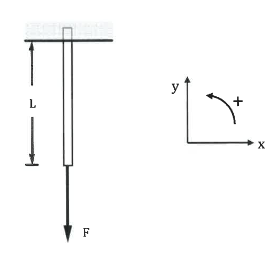
\includegraphics[scale=0.9]{fig1-rdm-0058.png}
\end{figure}

\medskip

Le barreau est encastré à son extrémité supérieure. On lui applique un effort $F = 285 \mathrm{~kN}$. Il s'allonge alors de $\Delta u = 3,8 \mathrm{~mm}$. Le barreau a une section carrée de $a=20 \mathrm{~cm}$ de côté et une longueur $L=6 \mathrm{~m}$. Les réponses seront dans un premier temps formulées de façon littérale puis en faisant l'application numérique.

\medskip

\begin{enumerate}
  \item Calculer la déformation unitaire du barreau.
  \item Déterminer la contrainte de traction subie par le barreau.
  \item Déterminer le module d'Young du matériau constituant le barreau.
\end{enumerate}

\finenonce{rdm-0058}
\finexercice


\end{document}
